\documentclass{article}
\usepackage{FinalYearProjectReport}

\usepackage[pdftex]{graphicx}
\graphicspath{{./}}
\DeclareGraphicsExtensions{.png}
\usepackage[final]{pdfpages}
\usepackage{hyperref}
\usepackage{underscore}
\usepackage{dblfloatfix}

\title {COMPSYS305 Mini Project}
\name {Hamish O'Neill and Roman Amor}
\address{Department of Electrical and Computer Engineering\\
University of Auckland, Auckland, New Zealand}

\hyphenation{and-roid}

\begin{document}

\maketitle

\abstract

This paper reviews the project undertaken for COMPSYS 305 at the University of Auckland in which a game was developed using Finite State Machine - Datapath design methodology in order to further the understanding and practical knowledge of VHDL of the students.
Through exploring the advanced options of using flash and mif files to implement images and sound, the students have taken the game further than the project requirements and produced an end product which is more enjoyable both to play and to look at.
This has both made the gaming experience much more enjoyable and considerably increased the student’s understanding of FPGA design and use.

\section{Introduction}

\subsection{The design specification}

The specification calls for a single player game to be developed using only digital logic on an FPGA. We are using the Terasic DE0 board which contains the Altera Cyclone III FPGA, Flash and SDRAM external memory, PS/2 mouse input, VGA screen output, LEDs, push buttons and DIP switches.

The game is played using the mouse. The player moves the mouse left and right to move their tank at the bottom of the screen. There are also AI-controlled tanks moving back and forth at the top of the screen. The player can press the mouse button to shoot a bullet, this bullet will move up the screen and if it touches an enemy tank the tank will be destroyed, causing it to respawn at a random location at the top of the screen. A second bullet cannot be shot until the bullet either hits a tank or goes off screen. As a basic requirement, the tanks and bullets should be represented by coloured rectangles displayed on the VGA monitor.

We have used the FSM-D design methodology, with a finite state machine drawn out using state transition diagram, and a datapath drawn out as a block diagram. This design was then implemented using behavioural VHDL descriptions that synthesise onto the FPGA. We have also made use of a couple of Python scripts, both custom made and modified from the internet, in order to create memory initialisation files tailored to our digital system from standard image and audio files.

\subsection{Contributions}

We took and heavily adapted an open source python script that takes .png files and converts them to .mif format. 
\url{https://github.com/Nananas/ImageToMif}

Other than that all of our extra tools have been developed in house.

All background images and sounds were obtained and modified under creative commons 0 licencing.

Tanks and bullet sprites and all modifications were done in house.

\section{The Game}

\begin{figure*}[!b]
\centerline{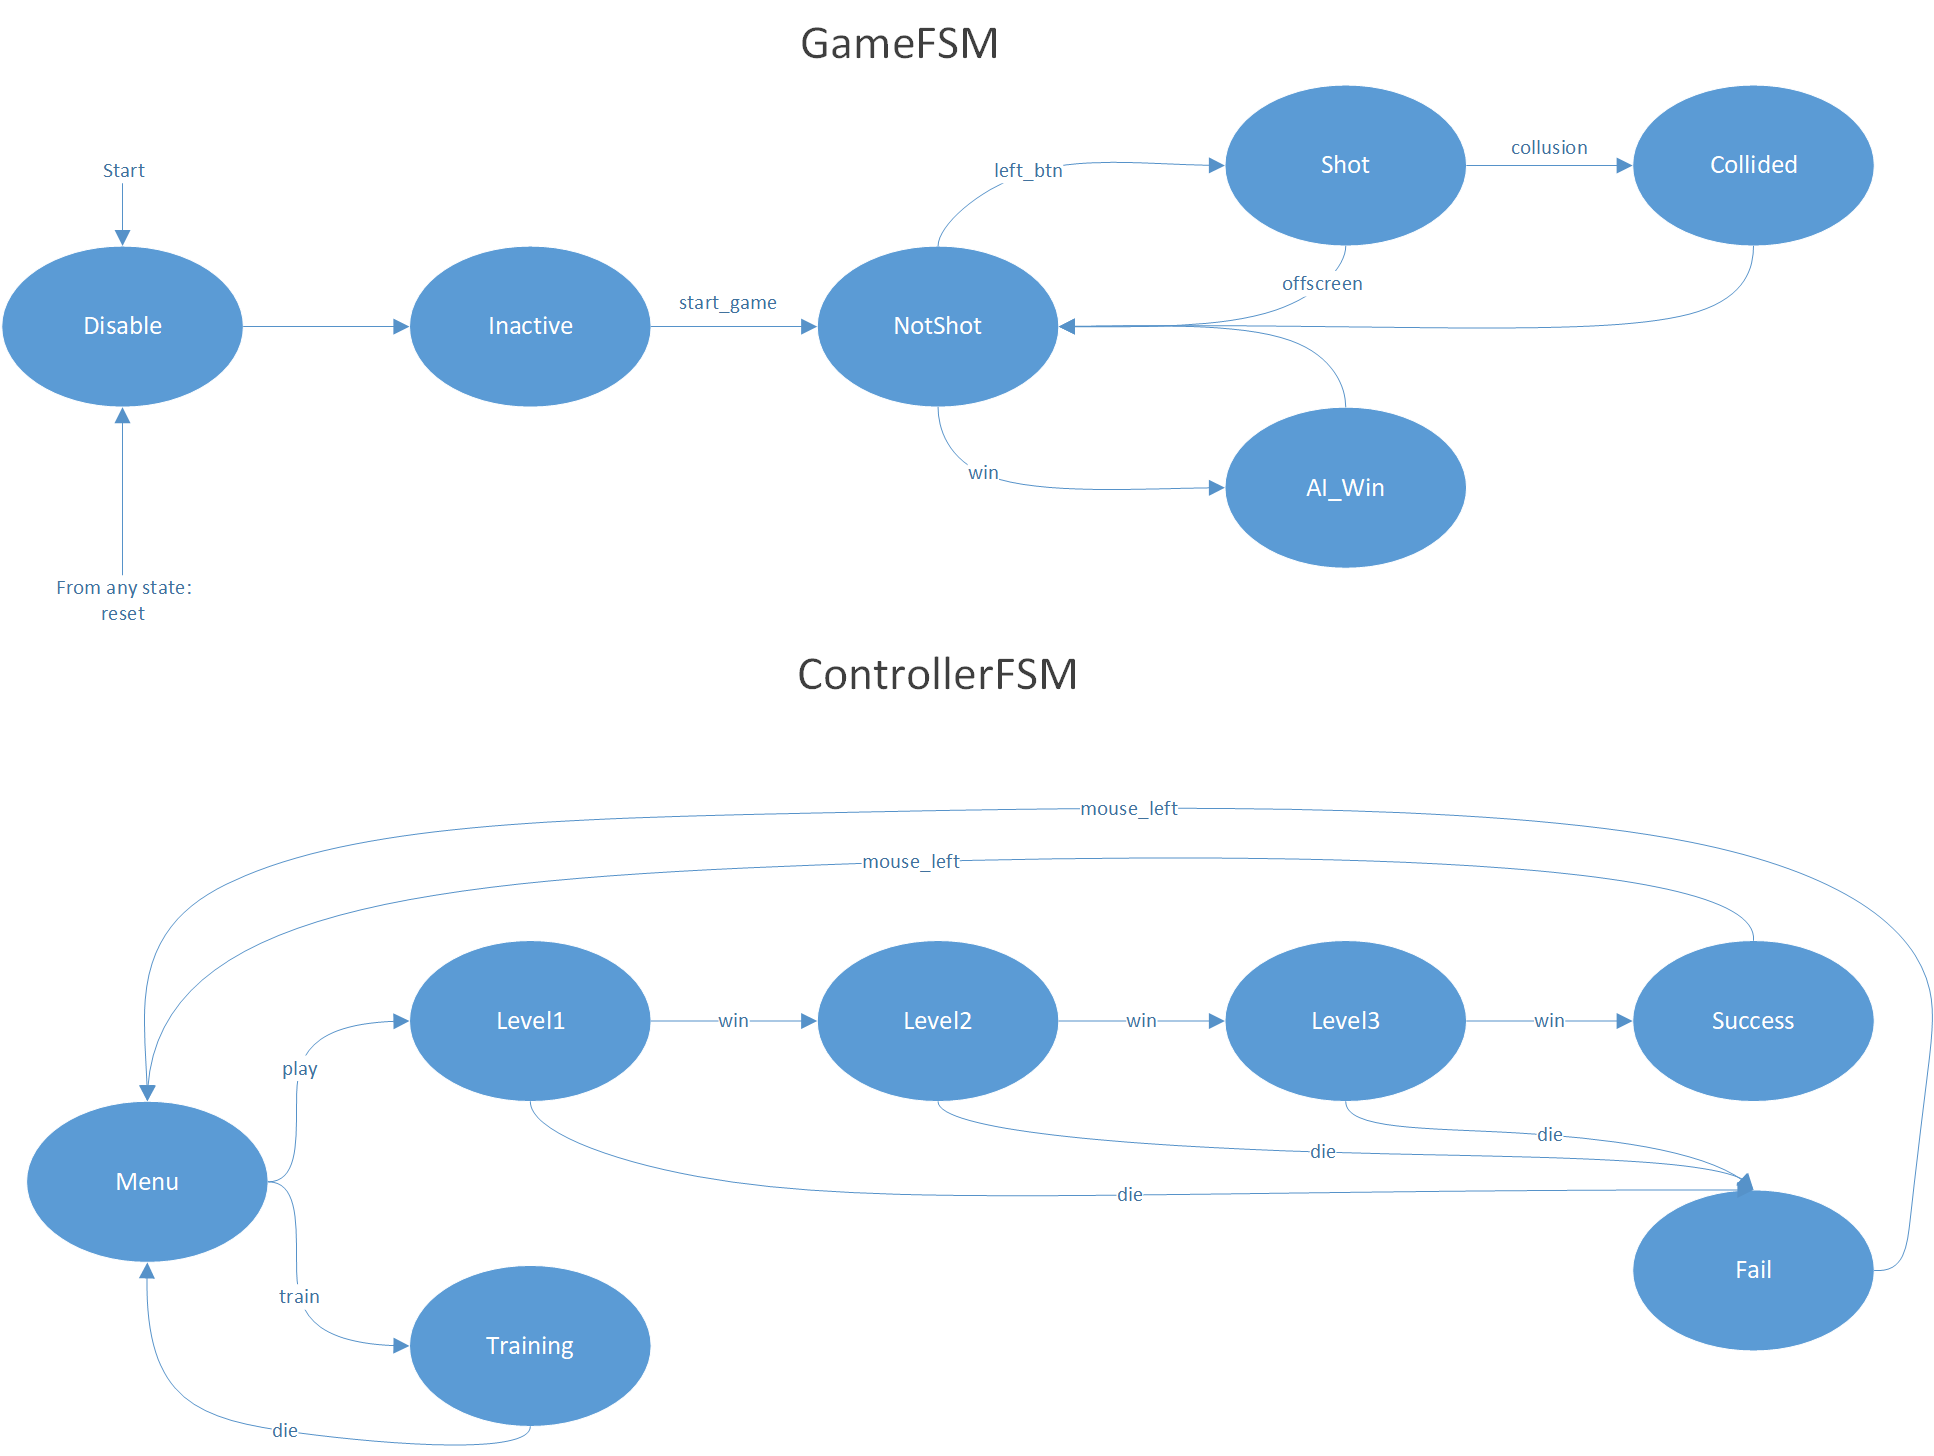
\includegraphics[height=4in]{FSMdiagram}}
\caption{Finite State Machines Used}
\label{fig:fsm}
\end{figure*}

\subsection{Rules and Features}

In addition to the basic game specifications, we have decided to implement a number of extra features. Firstly, we are using images with 4-bit colour as the graphics for the background, tanks and bullet instead of plain rectangles. We have also used audio tracks for both background music and sound effects.

Our design adds complexity to the basic game in a number of ways. There are multiple enemy tanks that travel left and right at different speeds. As the player scores more points, more tanks are added. As the tanks reach the edge of the screen they move down towards the user, and if they reach the bottom of the screen the user loses one life. Once the user loses all of their three lives, they lose the game.

For each time the user successfully kills a tank they are rewarded with one point. Once the user has accumulated 10 points they proceed to the next level. Subsequent levels will be aesthetically different with a different background image, and harder as there will be more tanks and they will be moving faster. If the user progresses through all the levels they win the game.

We also show the user their streak, which is how many consecutive successful shots they have made. This adds interest and competitiveness to the game. If the user reaches a streak of 5 they are rewarded with one extra life. When an enemy tank reaches the bottom of the screen, or the player misses with a shot, the streak resets to zero.

We are displaying the score, streak and lives remaining in the top right corner of the screen using text, and the lives are represented by a number of heart characters. The user is also be timed by a countdown timer and if the user takes longer than 30 seconds on any level they will automatically lose the game.

\subsection{Human-Computer Interfaces}

We have designed the game to rely as little as possible on the inputs on the DE0 board, and as such only have inputs here for the uses which are required in the project brief - reset functionality. All other inputs are provided using the mouse, both using a graphical user interface and using the various buttons on the mouse itself.

\subsection{How to Play}

The player starts the game by using the mouse to click on one of the 2 game modes, play mode or training mode.
The player will be presented a countdown timer and when it finishes, the game will begin. The player can then use the mouse and the left click mouse button to move their tank horizontally and fire bullets respectively. Both game modes will finish if the time runs out, however in play mode this will cause the player to lose the game. In the play mode, the player must get 10 points in each of the 3 levels in order to progress to the next. If they are able to complete all three before the time finishes, they will be presented a success screen.

On either the success or failure screens, the left mouse button can be used to get back to the main menu screen.

The player can press Button 2 on the DE0 board at any time in order to reset the game and return to the main menu screen.

The player can also press the middle mouse button at any time to toggle pause.

\begin{figure*}[!b]
\centerline{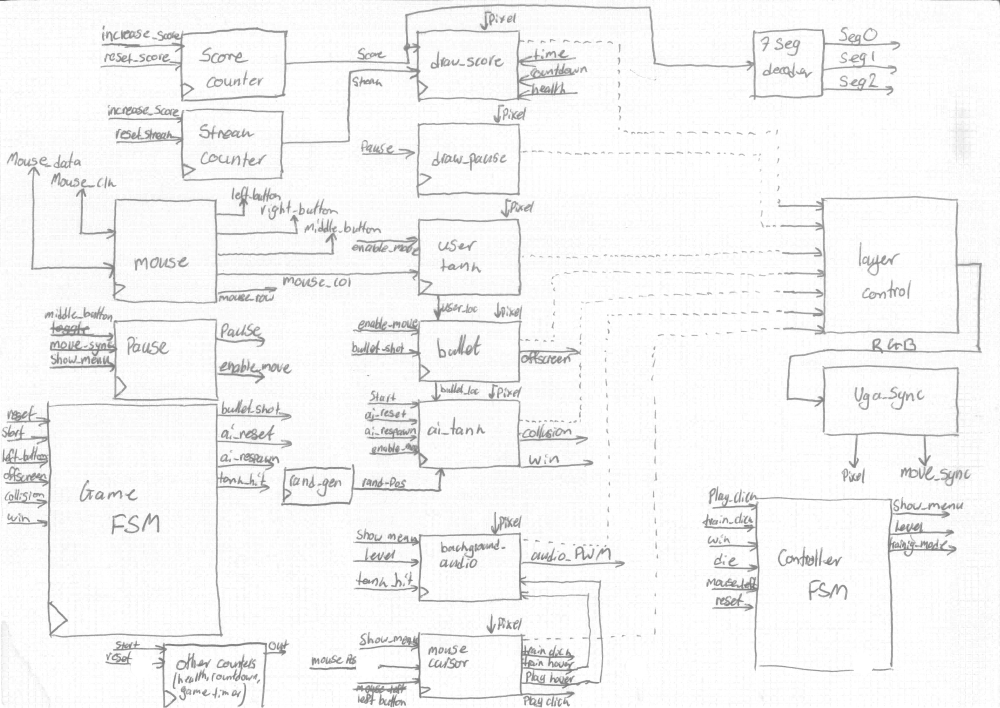
\includegraphics[height=4in]{blockDiagram}}
\caption{Block Diagram}
\label{fig:blockd}
\end{figure*}

\section{Implementation}

\subsection{Finite State Machines}

As per \ref{fig:fsm}, our design has two FSMs, ControllerFSM which coordinates the menu screen and level progression, and GameFSM which coordinates the movement and resetting of bullets and tanks within each game.

ControllerFSM starts in the Menu state where a menu screen is displayed by users. The show_menu output is used to enable the mouse pointer, disable other game objects and reset the GameFSM. Depending on where the user clicks the mouse button the datapath will assert the play or train signal. When play is asserted the state changes to Level1 and the game starts. The level is output to the datapath to determine which tanks are active, and the state directly determines which background image is displayed. The GameFSM will output the win or die signal. The win signal will causes the FSM to transition to Level2 and then Level3 once it is asserted again. From Level3 the win signal causes a transition to the Success state and the die signal causes a transition to the Fail state from all three level states. In both the Success and Fail state a background images with appropriate text is displayed and the a mouse click causes a transition back to the Menu state/screen. From Menu the train signal will alternatively take the user to the Training state where the trainingMode output will be set to high so the GameFSM will not let the user proceed to the next level. Once GameFSM asserts die the state returns to Menu.

Coming from the menu screen, GameFSM starts in the Disable state and asserts ai_reset to reset the positions of the AI controlled tanks and start the countdown timer. After one clock cycle it transitions to the Inactive state where it waits until the countdown timer finishes, which asserts start_game causing the FSM to transition to the NotShot state. In NotShot no special signals are asserted which means the user's tank and bullet is locked to the position of the mouse at the bottom of the screen. From here is the user clicks the left mouse button the FSM transitions to the Shot state. In Shot the bullet_shot signal is set high which latches the bullet x position to it’s current value and moves it upwards each redraw cycle. If the bullet exceeds the dimensions of the screen it will assert the off_screen signal and the state transitions back to Not Shot. If any of the tanks detect the bullet within their boundaries they will assert collision causing a transition to the Collided state. In Collided the increase_score and increase_streak outputs are pulled high to increment both counters, then on the next clock cycle the state transitions back to NotShot. If an AI tank reaches the bottom of the screen the win input will be high and the the state changes from NotShot to AI_Win where death and respawn will be asserted, causing the streak counter to reset and the tank that had reached to bottom to return to a random location at the top respectively. The next clock cycle the state returns to AI_Win.

\subsection{System Block Diagram}

Each visible game object has its own component in our datapath (see \ref{fig:blockd}, the user tank, bullet, multiple AI tanks and the background),. Internally each of these components has its own memory block (made from a combination of the M9K blocks built into the FPGA). They take in the current pixel row and column and use this to find the appropriate RGB values based on the location and size of the object they represent. The layer_control component takes in all these RGB values and displays them according to a priority list. The first bit of the RGB signal from each component indicates whether it is to be displayed at all for the current pixel row and column.

The user tank is given a signal enable_move from the FSM that determines if the users tank x position moves with the output from the provided mouse component or is latched (as is the case before the start of the game). The bullet works similarly with its location derived from the location of the user tank, until the bullet_shot signal is exerted by the FSM then its x location is latched and its y location is decremented each clock cycle so it appears to move upwards.

The AI controlled tanks start moving left and right at the start of the game when the start signal is exerted. The ai_tank components take in the bullet location and exert the collision signal when the bullet hits them. When they reach the bottom of the screen they exert the win signal. The FSM uses these signals to update the score/streak counters appropriately, then exerts the respawn signal which causes AI tanks to respawn in a new random location if they had been previously hit or reached the bottom of the screen.

The streak and score counters are incremented and reset by signals from the FSM, then they output a binary-encoded decimal that is displayed on the screen by the draw_score component using the provided character ROM. The score is also output to the 7 segment displays through a decoder.

\section{Results}

\subsection{Resource Consumption}

We are using 2543 logic elements, 558 of which are dedicated logic elements, to implement our digital logic. We are using 308k bits out of the 56 M9K blocks to store small sprite images, a buffer for the background image data read from the flash and the explosion sound effect.

We are storing all of our background images in the flash, as well as the background music. The flash must be read at half the rate of our pixel clock, so to manage this we are reading one row of flash data (for the new row) into the M9K buffer and one audio sample each horizontal sync  We have had some issues in being able to read the later addresses of this flash, so using the first 3.3MB of flash, we have 7 320x240px background images and around 30 seconds of background music.

\subsection{Timing Analysis}

According to the slow 1200mV model our maximum operating frequency is 62.0MHz, well above our clock speed of 50MHz. This means that the delay along our critical path is 16.1ns. This path is between the pixel_column output from the VGA sync component through our combination logic to the input of the memory for the AI tank images. We could break this critical path by registering the location of each AI tank (delaying location update by one clock cycle).

\section{Discussion and Future Work}

\subsection{Conclusion}

Developing this game has been a very beneficial for our knowledge of VHDL and general digital design ability. We have used it as an opportunity to experiment with the more technical aspects of the game by using graphics, flash memory and playing audio through PWM. Despite this we believe we have created a game that is simple yet enjoyable for a short play. We have impressed ourselves with how much we have been able to accomplish using just hardware design with zero software.

\subsection{Future Work}

In the future there are a number of improvements we would like to make. We would mostly like to improve the enjoyability and complexity of the game for the user. This could involve giving the AI tanks some kind of intelligence so they avoid the users and/or fire bullets back, reducing the user's health.

From a technical standpoint we would like to improve the graphics used. We would investigate using the SDRAM to buffer whole background images from the flash, allowing us to increase their resolution. As well as sound effects we would also like to show small visual animations on events such as collisions, implemented as a sequences of images for each sprite.

We would also like to implement a high score system. This might involve interfacing with a PS/2 keyboard so users can enter their name then writing the scores into the flash memory so they are persistent.

\end{document}
